\subsection{Разработка синтаксического анализатора}

В данном разделе необходимо выполнить разработку алгоритмов функционирования синтаксического анализатора.

Синтаксический анализ – процесс сопоставления последовательности токенов с формальной грамматикой языка.
Результатом работы синтаксического анализатора является абстрактное синтаксическое дерево (AST),
которое отражает синтаксическую структуру входной последовательности и содержит всю необходимую информацию для дальнейших этапов работы транслятора.

В задачу синтаксического анализа входит поиск и выделение основных синтаксических конструкций текста входной программы,
установление типа и проверка правильности каждой синтаксической конструкции, а так же представление их в виде AST.

Существует два основных метода синтаксического анализа:

\begin{itemize}
    \item нисходящий;
    \item восходящий.
\end{itemize}

В данном проекте реализован нисходящий анализатор, работающий по методу рекурсивного спуска,
известный как парсер Пратта, который впервые описал Вон Пратт в статье «Нисходящий парсер с операторным предшествованием».

Этот метод основан на идее приоритета операторов и обработке различных уровней приоритета в выражениях.
В парсере Пратта каждый оператор имеет свой уровень приоритета.
Операторы с более высоким приоритетом связываются с операндами сильнее, чем операторы с более низким приоритетом.
Значения приоритетов для каждого оператора разрабатываемого предметно-ориентированного языка показаны в таблице~\ref{t:operator_priority}.

\clearpage

\begin{table}[h!]
    \Large
    \caption{Приоритеты операторов}
    \label{t:operator_priority}
    \centering
    \begin{tabularx}{\textwidth}{|c|X|}
        \hline
        Приоритет & Операторы             \\
        \hline
        0         & Минимальный приоритет \\
        \hline
        1         & =                     \\
        \hline
        2         & | |                   \\
        \hline
        3         & \&\&                  \\
        \hline
        4         & == !=                 \\
        \hline
        5         & < > <= >=             \\
        \hline
        6         & + -                   \\
        \hline
        7         & * / \%                \\
        \hline
        8         & -x or !x              \\
        \hline
        9         & (                     \\
        \hline
        10        & [                     \\
        \hline
    \end{tabularx}
    \vspace{\bottompaddingoftable}
\end{table}

Для примера работы приоритета операторов рассмотрим пример построения AST для арифметического выражения: $3 + 1 * 4 * 6 + 8$.
Диаграмма, показывающая рекурсивные вызовы для формирования выражений к приведенному примеру изображена на рисунке~\ref{f:priorities}.

\begin{figure}[ht]
	\centering
	\vspace{\toppaddingoffigure}
	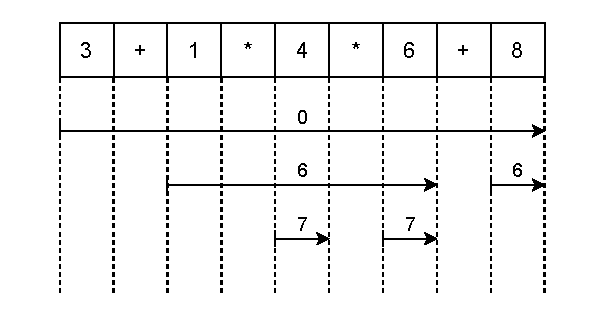
\includegraphics[width=0.7\textwidth]{structures/parser/priorities.pdf}
	\caption{Диаграмма рекурсивных вызовов}
	\label{f:priorities}
\end{figure}

Над стрелками обозначены приоритеты операторов, к которым относится эта стрелка.
В самом начале распознавания выражения значение приоритета равняется 0.
По мере обнаружения оператора, приоритет которого выше текущего алгоритм переходит на следующий уровень рекурсии.
По диаграмме видно, что справа от первого оператора «+» длинная стрелка с приоритетом 6, группирует члены умножения, так как операция умножения имеет больший приоритет, чем сложение.
Эта стрелка заканчивается перед последним «+», так как приоритет оператора, относящегося к этой стрелке не ниже приоритета последнего «+».
Другими словами, экземпляр выражения с более низким приоритетом ожидает результата формирования выражения с более высоким приоритетом.

Абстрактное синтаксическое дерево для данного примера приведено на рисунке~\ref{f:ast_example}.

\begin{figure}[ht]
	\centering
	\vspace{\toppaddingoffigure}
	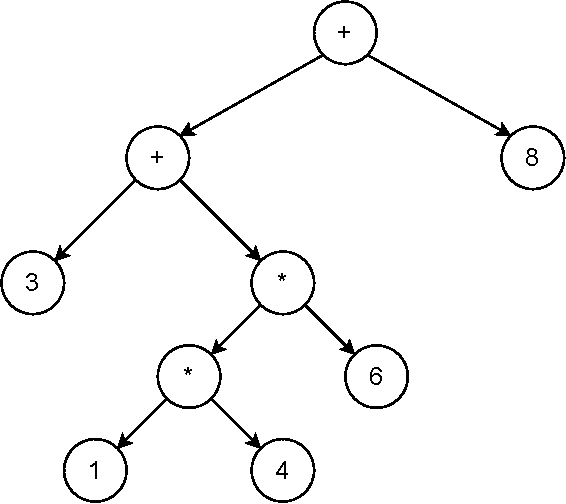
\includegraphics[width=0.7\textwidth]{structures/parser/ast_example.pdf}
	\caption{Абстрактное синтаксическое дерево}
	\label{f:ast_example}
\end{figure}

Некоторые схемы алгоритма построения абстрактного синтаксического дерева представлены на рисунках~\ref{f:parse_program}~-~\ref{f:parse_PrefixExpression}.

В данном разделе была выполнена разработка структурных решений и алгоритмов функционирования синтаксического анализатора.

\clearpage

\begin{figure}[!htp]
	\centering
	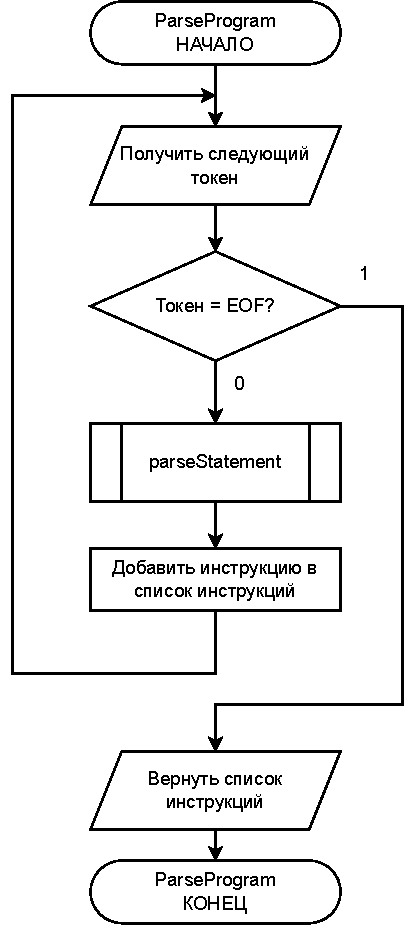
\includegraphics[width=0.5\textwidth]{structures/parser/parse_program.pdf}
	\caption{Схема алгоритма «Parse Program»}
	\label{f:parse_program}
\end{figure}

\clearpage

\begin{figure}[!htp]
	\centering
	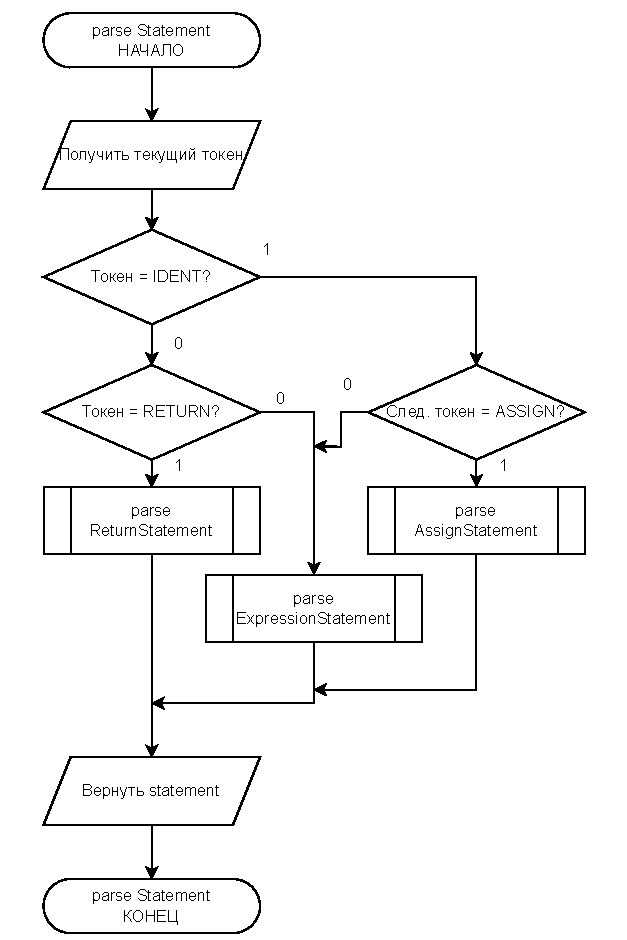
\includegraphics[width=0.7\textwidth]{structures/parser/parse_statement.pdf}
	\caption{Схема алгоритма «parse Statement»}
	\label{f:parse_statement}
\end{figure}

\clearpage

\begin{figure}[ht]
	\centering
	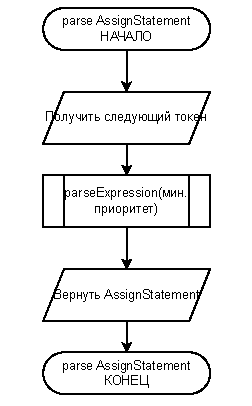
\includegraphics[width=0.4\textwidth]{structures/parser/parse_assignStatement.pdf}
	\caption{Схема алгоритма «parse AssignStatement»}
	\label{f:parse_assignStatement}
\end{figure}

\begin{figure}[!htp]
	\centering
	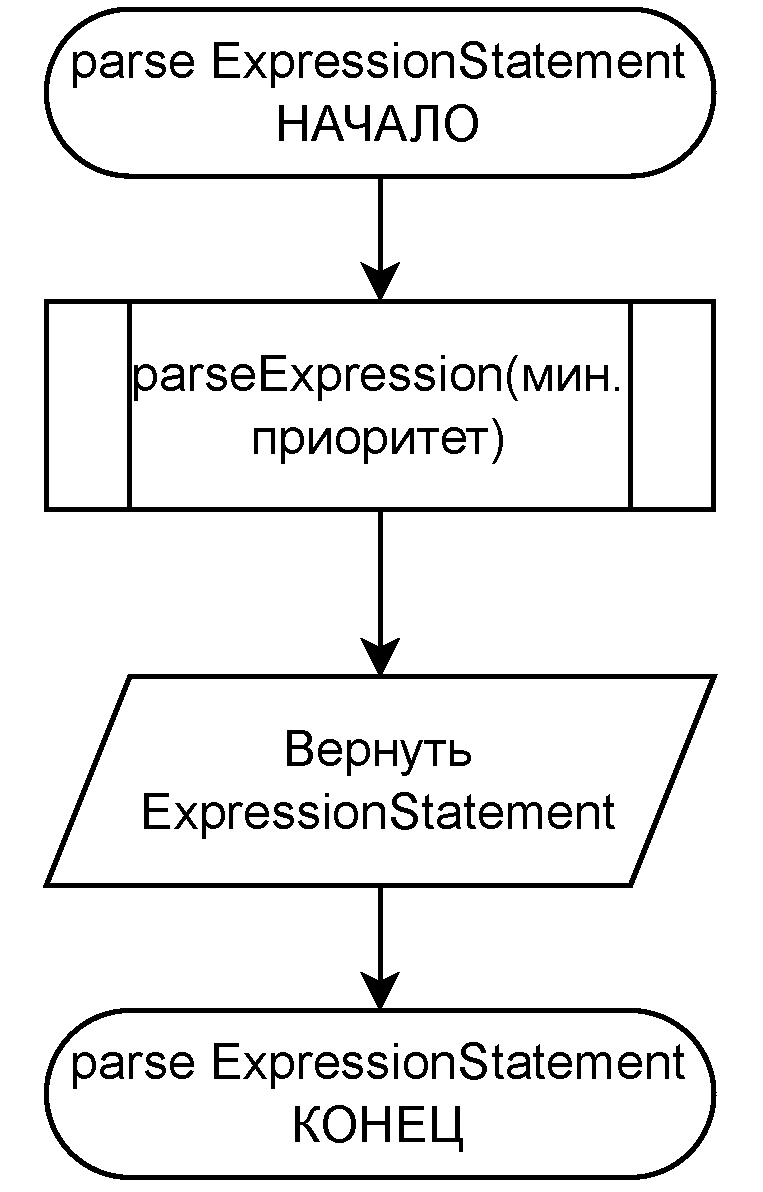
\includegraphics[width=0.3\textwidth]{structures/parser/parse_expressionStatement.pdf}
	\caption{Схема алгоритма «parse ExpressionStatement»}
	\label{f:parse_expressionStatement}
\end{figure}

\begin{figure}[!htp]
	\centering
	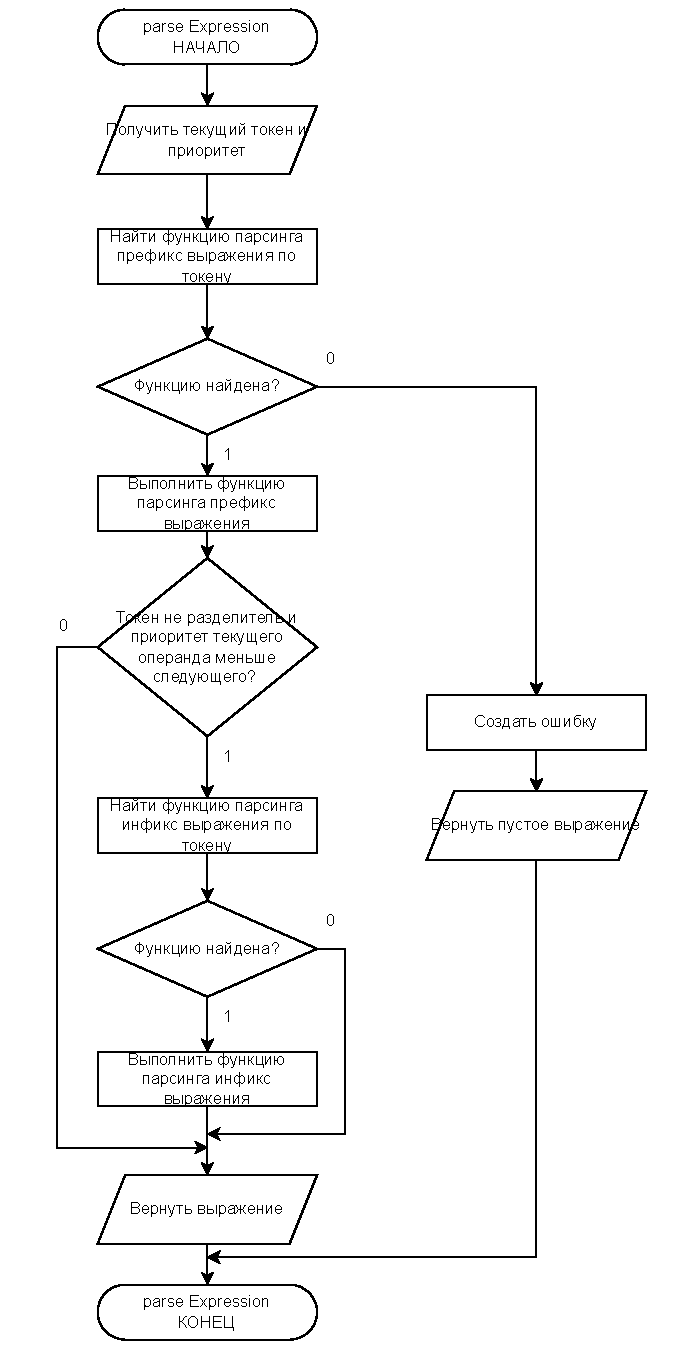
\includegraphics[width=0.65\textwidth]{structures/parser/parse_Expression.pdf}
	\caption{Схема алгоритма «parse Expression»}
	\label{f:parse_Expression}
\end{figure}

\clearpage

\begin{figure}[!htp]
	\centering
	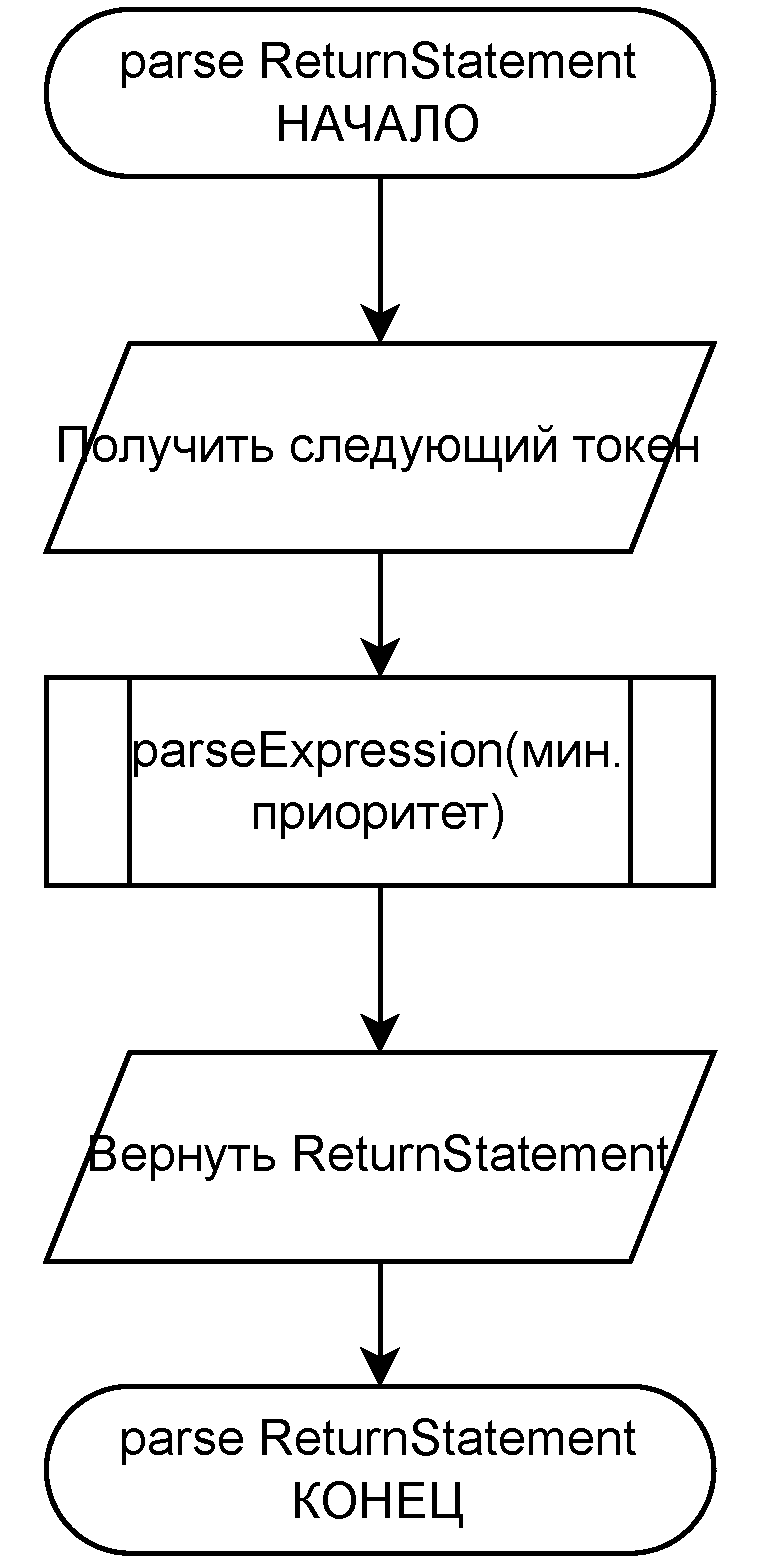
\includegraphics[width=0.3\textwidth]{structures/parser/parse_returnStatement.pdf}
	\caption{Схема алгоритма «parse ReturnStatement»}
	\label{f:parse_returnStatement}
\end{figure}

\begin{figure}[!htp]
	\centering
	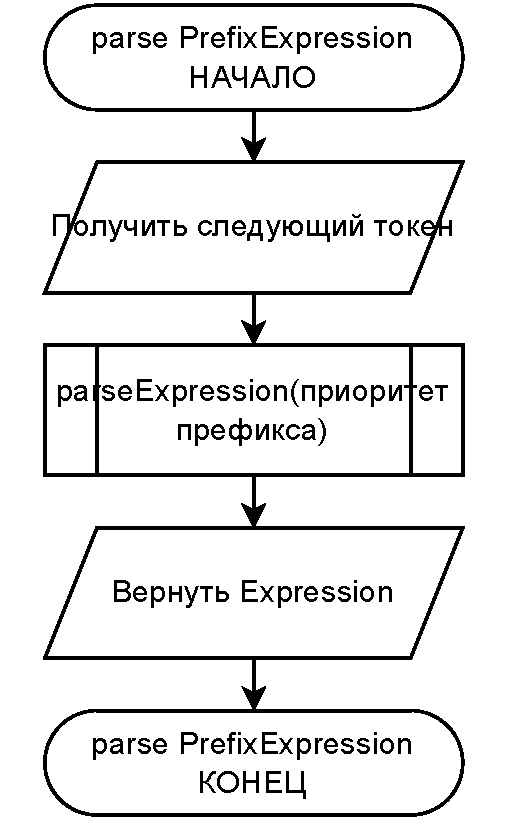
\includegraphics[width=0.3\textwidth]{structures/parser/parse_PrefixExpression.pdf}
	\caption{Схема алгоритма «parse PrefixExpression»}
	\label{f:parse_PrefixExpression}
\end{figure}

\clearpage

